\documentclass[11pt, oneside]{article}   	% use "amsart" instead of "article" for AMSLaTeX format
\usepackage{geometry}                		% See geometry.pdf to learn the layout options. There are lots.
\geometry{letterpaper}                   		% ... or a4paper or a5paper or ... 
%\geometry{landscape}                		% Activate for rotated page geometry
%\usepackage[parfill]{parskip}    		% Activate to begin paragraphs with an empty line rather than an indent
\usepackage{graphicx}	
\graphicspath{ {./images/} }			% Use pdf, png, jpg, or eps§ with pdflatex; use eps in DVI mode
								% TeX will automatically convert eps --> pdf in pdflatex		
\usepackage{amssymb}

%SetFonts

%SetFonts


\title{Consumer Delinquency Rates and Federal Debt}
\author{Adi Jahic, Supreet Bhavireddy, Jenna Peters}
\date{October 2021}		
				% Activate to display a given date or no date

\begin{document}
\maketitle	
\section{Introduction}
The acceleration of the United States Federal Debt over the past two decades has become an extremely political issue. This is because Federal Debt is largely controlled by fiscal policy. As the political climate in the US becomes more polarized, fiscal policy and the Federal Budget become more about political alignment than economic implications. Our research seeks to peel back the layer of politics, and analyze a metric that influences policy on the Federal Budget, thus influencing Federal Debt.


Looking at the time series for Federal Debt as a percentage of GDP (referred to simply as debt),  during recessionary periods, we saw an acceleration during recessionary periods (Figure 1). This was expected, as fiscal policy tends to increase government spending during recessionary periods in order to recover. However, this led to the idea that Federal Debt would rise in periods of low economic health, even if there wasn't necessarily a full blown recession. A metric that measures the health of an economy could possibly forecast Federal Debt.

\begin{figure}[h]
\centering
\begin{minipage}{.5\textwidth}
  \centering
  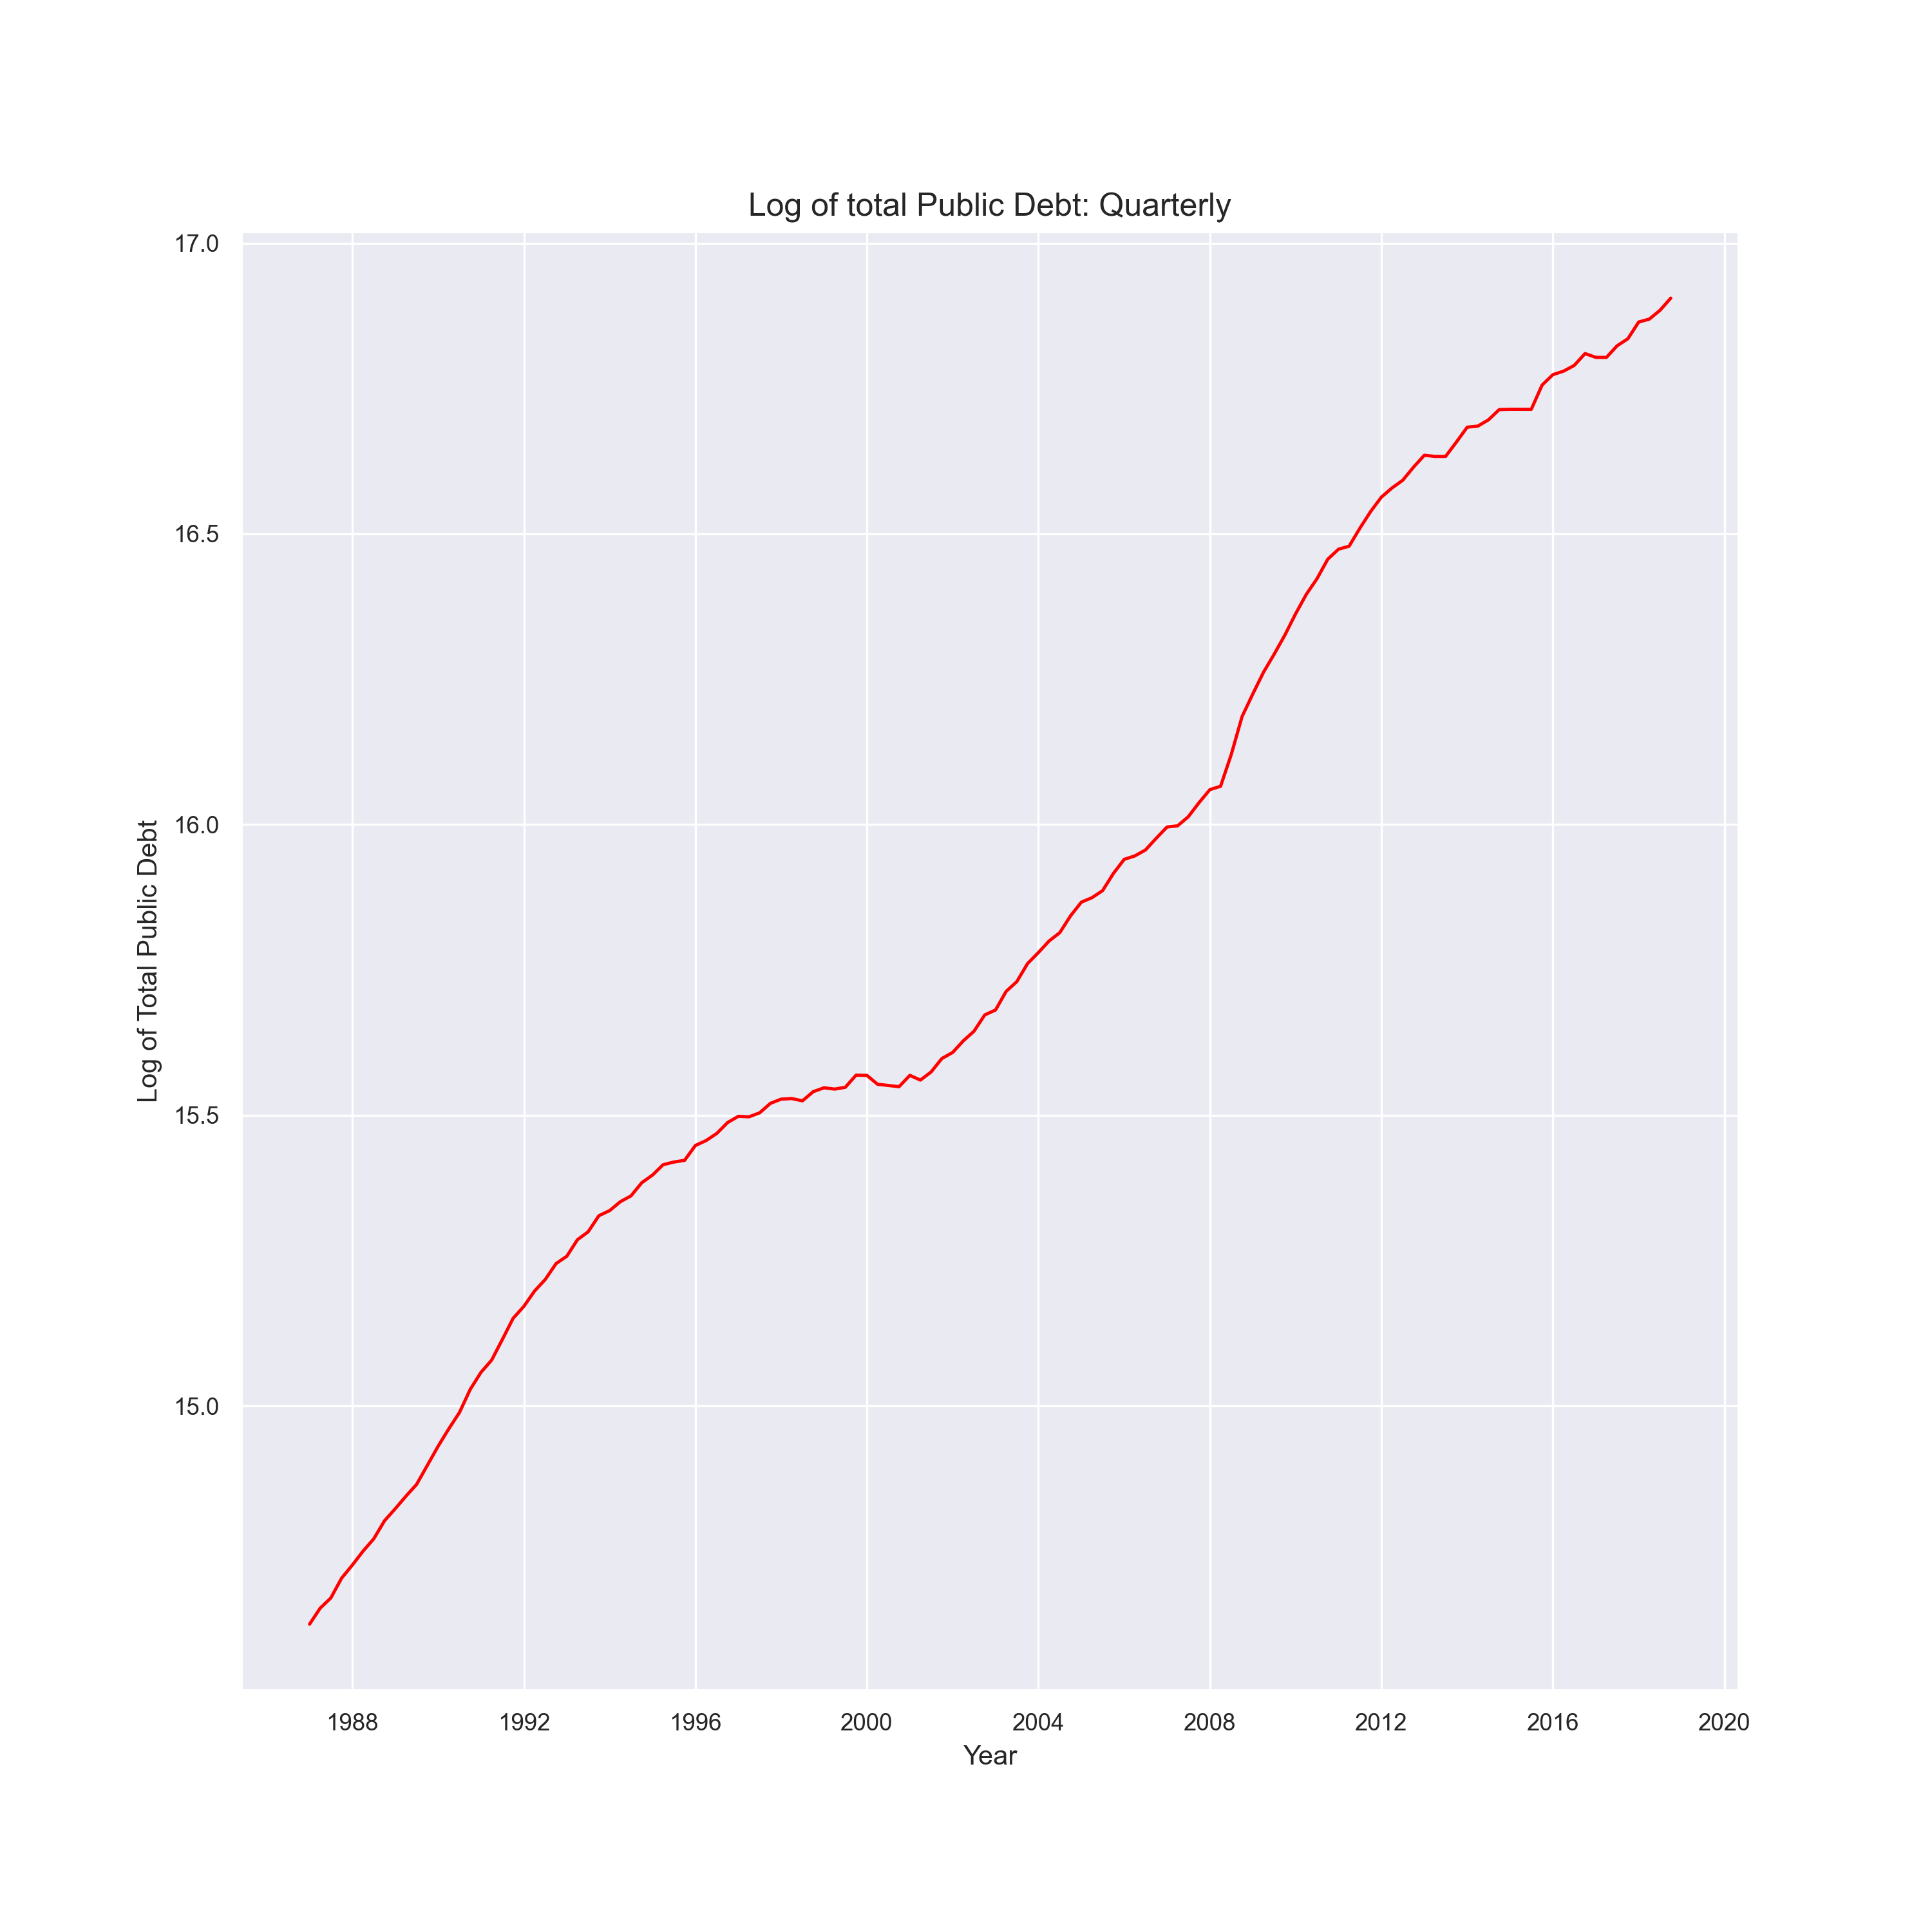
\includegraphics[width=.8\linewidth]{lndebt_graph}
  \caption{Log of Total Public Debt}
  \label{fig:test1}
\end{minipage}%
\begin{minipage}{.5\textwidth}
  \centering
  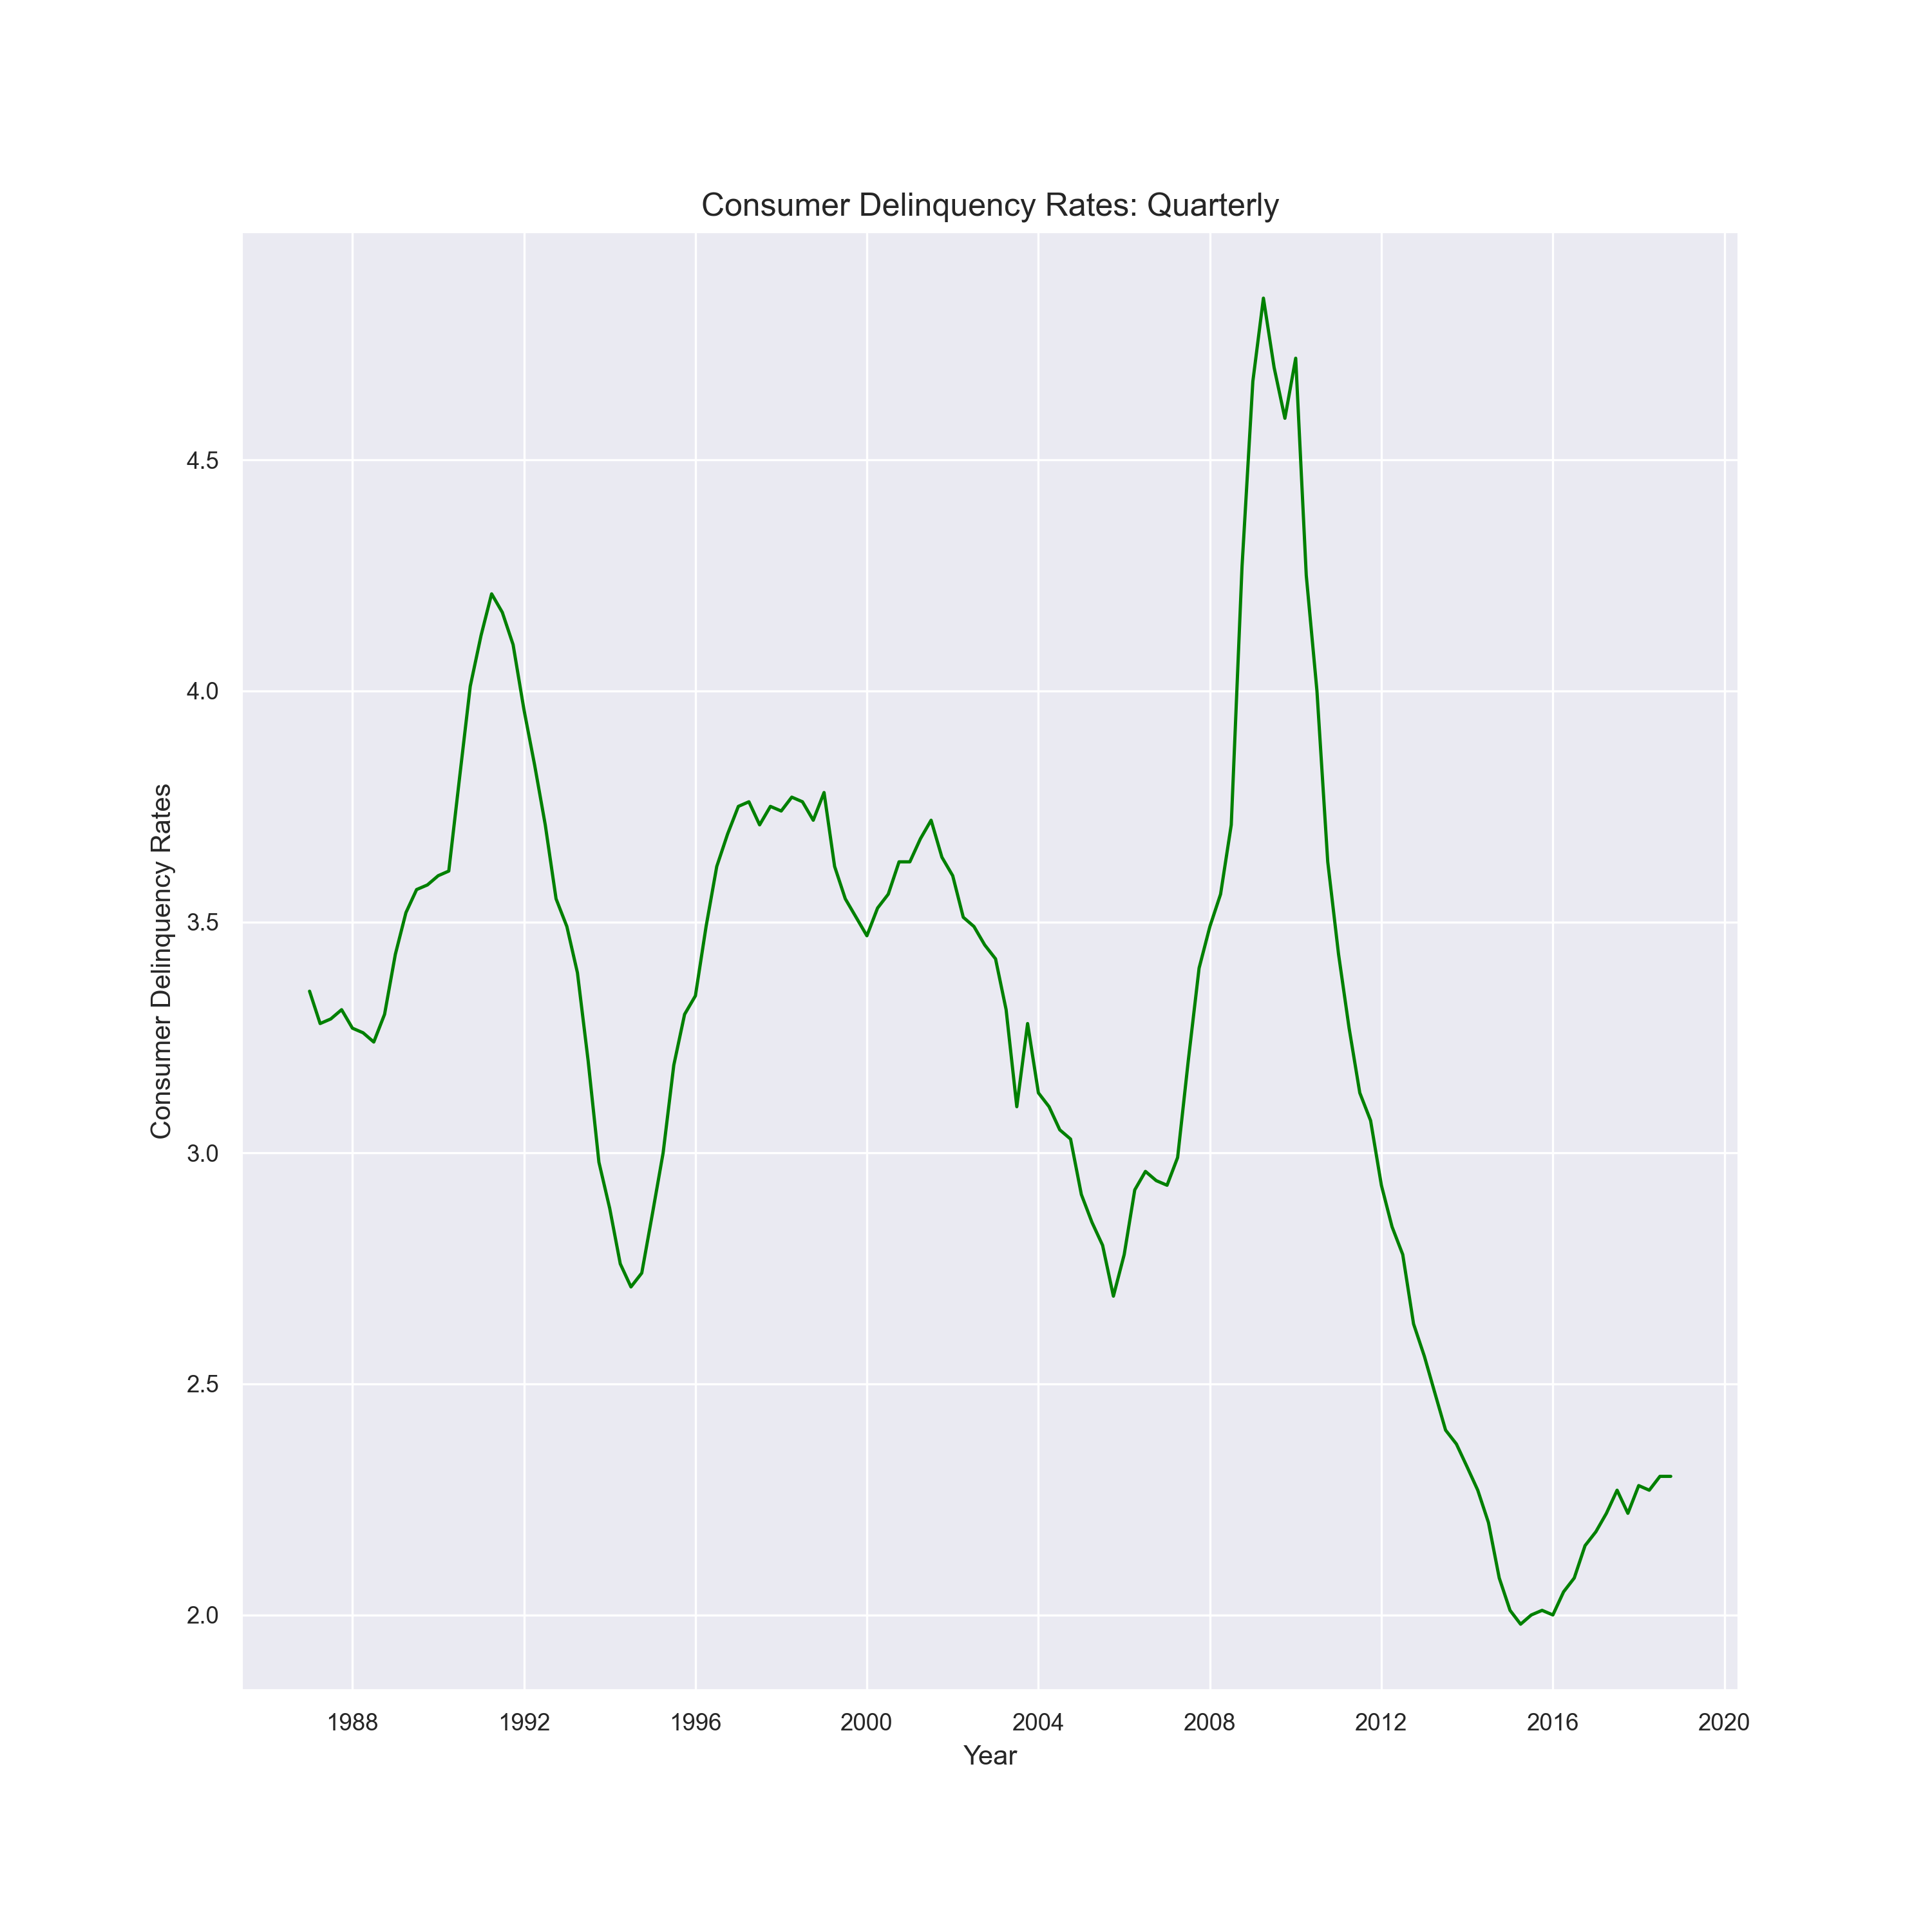
\includegraphics[width=.8\linewidth]{rates_graph}
  \caption{Consumer Delinquency Rates}
  \label{fig:test2}
\end{minipage}
\end{figure}

The inspiration behind the metric we chose to measure economic health came from the story of hedge fund manager Michael Burry and his foresight of the 2008 Housing Market Crash. One of the main indicators to him that the crash was coming, was the high delinquency rates on subprime consumer mortgages. Mortgage delinquency rates were on the rise before the recession hit (Figure 2). Using consumer delinquency rates on credit card, mortgage, and aggregate consumer debt, we hypothesized we could forecast Federal Debt. The intuition was that if consumers are struggling, delinquency rates rise, and fiscal policy may respond by increasing spending, even if the economy isn't necessarily in a recessionary period. Our research will explore the relationship between consumer delinquency rates (referred to as del rate) and Federal Debt and if the Consumer Delinquency rates are good forecasters of Federal Debt.



\section{Literature Review}
	The idea to use a time series metric to forecast another came from the academic paper \emph{"The Effects of Oil Price Volatility on Ethanol, Gasoline, and Sugar Price Forecasts"} by Lucio Guido and Tapia Carpio. Guido and Carpio essentially analyzed the effect of oil prices on sugar, gasoline, and ethanol price forecasts using a VECX model. Our research similarly will focus on modeling each time series, and then using a VAR model to interpret their relationship. However, their model fails to consider breaks in the series. We will improve upon their methodology by identifying breaks. 
	
	Why mortgage delinquency rates rose so quickly before the 2008 recession --- ultimately leading to the housing market crash --- is discussed in Atif Mian and Amir Sufi's paper \emph{The Consequences of Mortgage Credit expansion: Evidence from the U.S. Mortgage Default Crisis}. They concluded that a rise in mortgage credit to subprime neighborhoods was the main cause for high mortgage delinquency rates, and following defaults. Mortgage credit grew among subprime neighborhoods, yet there was negative income growth.
	
	In Mokhtarul Wadudb Huson Joher Ali Ahmeda, and Xueli Tangc's paper \emph{Factors Affecting Delinquency of Household Credit in the U.S.: Does Consumer Sentiment Play a Role?}  they conclude if consumers have optimistic sentiment about current and future economic conditions, then credit default rates will go up. They infer that this is due to "over-optimism", that consumers are too positive about the future, and spend in excess, then default rates go up. 
	
	Both papers described a pattern of consumer or creditor optimism, followed by increased volume of credit, and then a subsequent increase in delinquency rates among consumers due to overoptimism, which can lead to a recession like in 2008, or general poor economic health. Our hypothesis is then, that consumer optimism and investment are thus poor forecasters of economic health, and delinquency rates better capture how consumers are faring. If delinquency rates better capture the financial health on consumers, will delinquency rates impact fiscal policy? Specifically, will delinquency rates impact policy makers decision to increase spending and thus increasing Federal Debt?

\section {Model Selection}

Since we are working with two different variables with the intention of co-integrating them, we had to be very deliberate in our choosing of a model for each variable.

With any time series data, it's crucial to ensure stationarity in the data before proceeding. Looking at the data, it's clear that stationarity isn’t achieved for either variable as there isn’t a constant mean nor a constant variance. We ran conventional unit root tests, such as Augmented-Dickey- Fuller (ADF), Phillips-Perron (PPerron), and the Generalized-Dickey-Fuller (DF-GLS), to test for the existence of unit roots which would tell us if this data is potentially a random-walk or is trend stationary. The ADF tests for unit roots while also providing an estimate for a trend in the data, if it exists. For both debt and del rate, we ran the test sequentially, beginning with max lags of ten to a lag of just one, and for each test we could not reject the null hypothesis of a unit root meaning the data was a random walk with or without drift, but the tests also did not provide us with a statistically significant trend variable. This led us to believe that both variables were difference stationary. 

Therefore, we took the first difference of both variables. The following graphs present the first difference of both variables:


\begin{figure}[h]
\centering
\begin{minipage}{.5\textwidth}
  \centering
  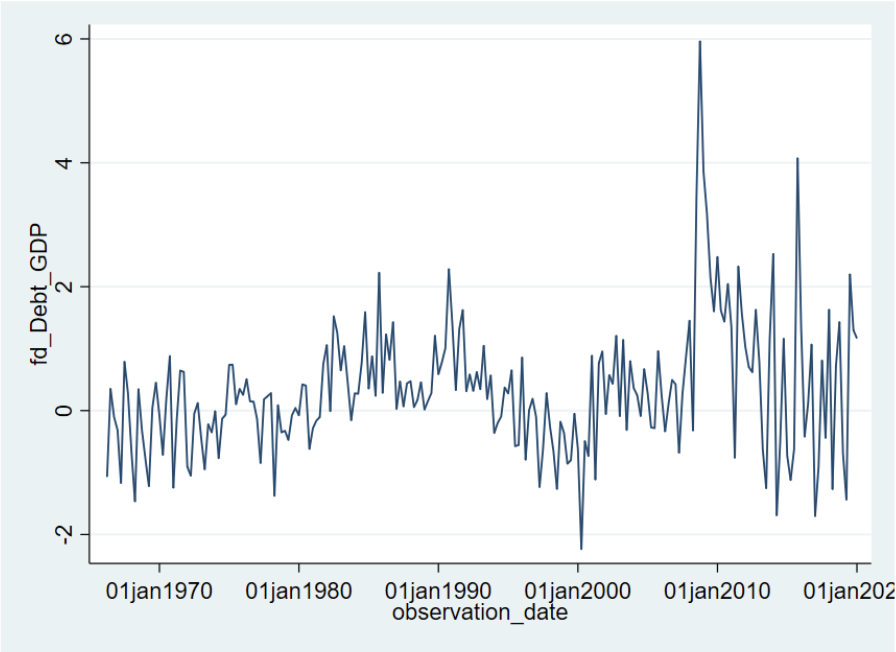
\includegraphics[width=.8\linewidth]{fd_debt}
  \caption{First Difference of Debt}
  \label{fig:test1}
\end{minipage}%
\begin{minipage}{.5\textwidth}
  \centering
  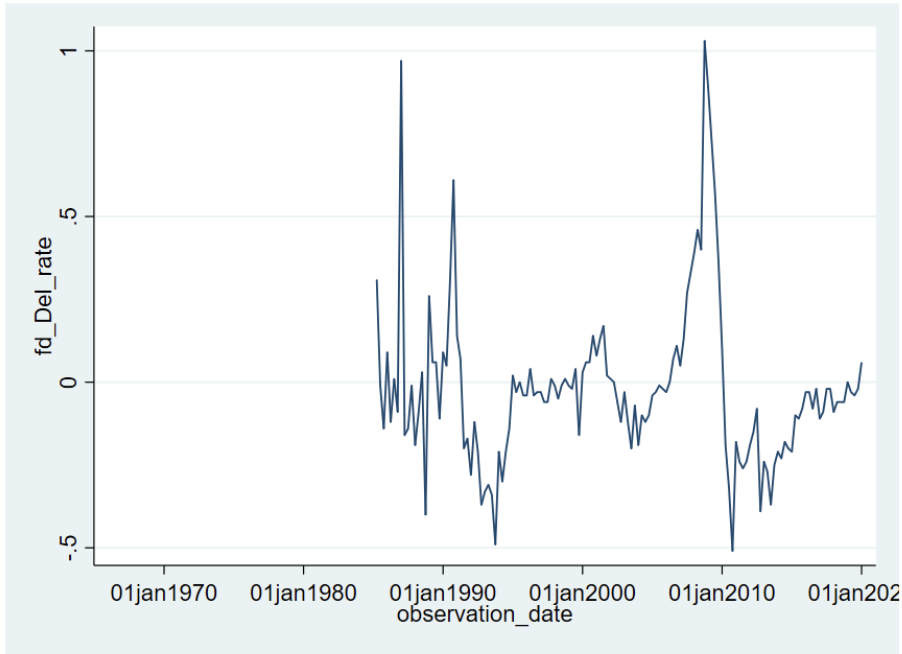
\includegraphics[width=.8\linewidth]{fd_rates}
  \caption{First Difference Delinquency Rates}
  \label{fig:test2}
\end{minipage}
\end{figure}


The data now looks as though it could be stationary. We run the ADF again, with max lags of ten and find that it is statistically significant at the maximum lags for both variables. Again, no statistically significant trend is found. We continued by running both PPerron and the DF-GLS which gave us the same result. 

We then needed to choose the most accurate model for each variable. Let’s begin with the first difference of debt. We began by finding the auto-correlation function (ACF) and the partial auto-correlation function (PACF) along with the “corrgram,” which are all different methods to determine the number of lags to which a variable is correlated. Essentially, these advise us on the number of lags which we should include in the model. All of these methods suggested just one lag with borderline significance in the next two was the best possible model. To confirm this, and decide between the auto-regressive, AR, or moving average, MA we checked the information criteria, AIC or BIC, for each of these options with one, two, or three lags. These information criteria test “accuracy” of a model, and it is ideal if both criteria suggest the same model, which, in this case, it did with the ar(1) model. This is consistent with what the ACF and PACF suggested. The model is as follows:

\[Y_{t} = 0.312 + 0.399Y_{t-1} + e_{t}\]


Afterwards, we ran the same process to find the model for the first difference of the del rate. For this model, however, the ADF suggested that the second lag may also be significant, so we expected a model consisting of two lags. We checked the ACF and PACF along with the “corrgram” in STATA and found that the lags seemed to only be strongly significant for the first two lags, and on the border of significance for the next five. We then considered the information criteria, AIC and BIC, for up to five lags in both AR, and MA, forms. Both criteria suggested that an AR(2) model, an auto-regressive model with two lags, was the best model, which is consistent with the ACF/PACF. 
The model is as follows: 

\[X_{t} = 0.0475_{t-1} + 0.287X_{t-2} + e_{t}\]


To test the strength of the models, we found the predicted values of each variable then found the root mean square error of each. This value was about 0.8 for debt and 0.9 for del rate. 

\section {Next Steps and Future Paper Goals}

One of our immediate next steps is to explore the precision of our time series model by testing the forecasting’s accuracy against actual observations for both debt and delinquency rates. Doing so lets us develop a better understanding of where our model’s shortcomings lie and how to interpret the underlying biases which are ever present within the model. From there, we will continue towards our goal of understanding how total federal debt impacts future delinquency rates. Following the procedure of Guido in his oil volatility paper, we will compare the time series models visually to observe similarities in debt and delinquency activity (barring structural breaks). Since both federal debt and delinquency rates react to their economic situation, understanding the time periods where both react in manner befitting a relationship will give us an understanding of what situations result in debt impacting delinquency rates in different manners.

To further develop our findings with our time series model, we will naturally have to consider the structural breaks that are present in the data series. Our first step will be to identify the breaks. Upon identifying the structural breaks we expect to use the Yabu Perro test developed in 2008 by the two aforementioned econometricians. The Yabu Perron test allows us to more accurately test flexible nonlinear deterministic trends, of which we concluded we have given our above work in detrending our data series (Perron et al. 2015). After using the Yabu Perron test, we will use the Kim Perron test to better develop useful insights on our data without structural breaks. Although we will account for structural breaks that occur during the series’ periods of observations, our intention will be to not use the latter quarterly periods since COVID-19 is an unprecedented shock for which there is no legitimate reference to properly account for in time series analysis. 

While we have the above autoregressive models, our goals make it clear that a vector autoregressive model would be helpful in further understanding the intricacies of how current and past debt interplays with past delinquency rates to develop future delinquency rates (Sims 1980). As further proof we can look at Guido’s research on oil volatility again to see that the bulk of his analysis on oil volatility implications on sugar, ethanol, and gasoline is done with a vector autoregressive model. To this objective, the previous tests we ran to detrend the time series will serve as a valuable starting point. From here the next steps will be to run stability tests and test various vector models by running model fitting tests on the different models to determine the ideal number of vector autoregressive lags. Another incentive to explore the vector autoregressive model further is that the model actively rewards the possibility to expand our use of delinquency rates from all loans to include the major types of  delinquency rates (mortgage, loan, auto, and credit delinquencies). As we add more equations we include in our model’s matrices, our information criterion becomes increasingly accurate in finding ideal fits for the vector autoregressive model while also accurately portraying the true relationship between debt and all delinquency rates as well. 




%\section{}
%\subsection{}



\end{document}  